\documentclass[11pt]{article}
\usepackage{amssymb,amsmath,amsthm,graphicx}
\usepackage{fancyhdr}

\def\shownotes{1}   % set 1 for version with author notes
                    % set 0 for no notes



%uncomment to get hyperlinks
%\usepackage{hyperref}

%%%%%%%%%%%%%%%%%%%%%%%%%%%%%%%%%%%%%%%%%%%%%%%%%%%%%%%%%%%%%%
%Some macros (you can ignore everything until "end of macros")

\topmargin 0pt \advance \topmargin by -\headheight \advance
\topmargin by -\headsep

\textheight 8.9in

\oddsidemargin 0pt \evensidemargin \oddsidemargin \marginparwidth
0.5in

\textwidth 6.5in

%%%%%%

\providecommand{\vs}{vs. }
\providecommand{\ie}{\emph{i.e.,} }
\providecommand{\eg}{\emph{e.g.,} }
\providecommand{\cf}{\emph{cf.,} }
\providecommand{\etc}{\emph{etc.} }

\newcommand{\getsr}{\gets_{\mbox{\tiny R}}}
\newcommand{\bits}{\{0,1\}}
\newcommand{\bit}{\{0,1\}}
\newcommand{\Ex}{\mathbb{E}}
\newcommand{\eqdef}{\stackrel{def}{=}}
\newcommand{\To}{\rightarrow}
\newcommand{\e}{\epsilon}
\newcommand{\R}{\mathbb{R}}
\newcommand{\N}{\mathbb{N}}
\newcommand{\Gen}{\mathsf{Gen}}
\newcommand{\Enc}{\mathsf{Enc}}
\newcommand{\Dec}{\mathsf{Dec}}
\newcommand{\Sign}{\mathsf{Sign}}
\newcommand{\Ver}{\mathsf{Ver}}

\providecommand{\mypara}[1]{\smallskip\noindent\emph{#1} }
\providecommand{\myparab}[1]{\smallskip\noindent\textbf{#1} }
\providecommand{\myparasc}[1]{\smallskip\noindent\textsc{#1} }
\providecommand{\para}{\smallskip\noindent}


\newtheorem{theorem}{Theorem}
\theoremstyle{definition}
\newtheorem{ex}{Exercise}
\newtheorem{definition}{Definition}

%%%%%%%  Author Notes %%%%%%%d
%
\ifnum\shownotes=1
\newcommand{\authnote}[2]{{ $\ll$\textsf{\footnotesize #1 notes: #2}$\gg$}}
\else
\newcommand{\authnote}[2]{}
\fi
\newcommand{\Snote}[1]{{\authnote{Solution}{#1}}}
\newcommand{\Inote}[1]{{\authnote{Solution}{#1}}}
\newcommand{\Ichanged}[1]{{\authnote{Changed}{#1}}}
%%%%%%%%%%%%%%%%%%%%%%%%%%%%%%%%%

\newcommand{\VAR}{\mathrm{VAR}}



% end of macros
%%%%%%%%%%%%%%%%%%%%%%%%%%%%%%%%%%%%%%%%%%%%%%%%%%%%%%%%%%%%%%


% page counting, header/footer
\usepackage{fancyhdr}
\pagestyle{fancy}
\lhead{\footnotesize \parbox{11cm}{CS455, Boston University, Fall 2015} }
\rhead{Erik Brakke}
\renewcommand{\headheight}{24pt}

\begin{document}

\title{Homework 2}
\author{Erik Brakke}
\maketitle

\thispagestyle{fancy}
 
 
\section*{Answer 1}

\begin{enumerate}
\item[P9.] $\delta = .85Mb/15Mbps = .057sec$\\
$\beta = 16 req/sec$
$\delta / (1 - \delta\beta) = .056 / (1 - .912) = .6$\\
Total average response time = $3 + .6 = 3.6$ seconds\\
\newline
$\delta\beta = 16 * .057 * .4 = .365$\\
$\delta / (1 - .365) = 3.09sec$\\
Total response time = $.4(3.09) + .6(0) = 1.23sec$\\

\item[P10.] Parallel downloads via parallel instances for non-persistant HTTP would not make sense in this case\\
Parallel or not, all of the objects must be downloaded which will take $(11 * 100,000)/150 = 7333.34$ transmitting at full capacity\\
Because we are using non-persistant HTTP, we can only recieve one object with each connection we setup.  We cannot get around the fact that we will have to make 11 different connections to the server.  If we do this in parallel, the RTT and object download time all increase because each connection only has a fraction of the total bandwidth.  Running in parallel is no different than running serial connections (because we will never imporove on overhead or download time)\\
\newline
Now let's consider persistant HTTP.  The gains will only be in the amount of overhead that we save.\\
We have 1 RTT (2.67 seconds) to establish the connection with the server\\
We then have to wait for the first object to download (2.67 seconds + 666.67 seconds)\\
After this we can request all 10 embedded objects (2.67 + 666.67) * 10\\
This is a total time of 7365.41 seconds\\
We've saved 26.7 seconds by not having to instantiate a new connection for every object.  This is an insignificant gain compared to how long it takes to download the objects\\

\item[P22.]
$D_{cs} = max\{\frac{NF}{u_s}, \frac{F}{d_{min}}\}$\\
$D_{p2p} = max\{\frac{F}{u_s},\frac{F}{d_{min}},\frac{NF}{u_s + \sigma_1^n u_i}\}$\\
F = 15,000,000 Kbits\\
$u_s$ = 30,000 Kbits/s\\
\begin{tabular}{|c|c||r|r|}
\hline
N & u & $D_{cs}$ & $D_{p2p}$\\
\hline
10 & 300kbps & 7500 & 7500\\
10 & 700kbps & 7500 & 7500\\
10 & 2000kbps & 7500 & 7500\\
100 & 300kbps & 50000 & 25000\\
100 & 700kbps & 50000 & 15000\\
100 & 2000kbps & 50000 & 7500\\
1000 & 300kbps & 500000 & 45455\\
1000 & 700kbps & 500000 & 20548\\
1000 & 2000kbps & 500000 & 7500
\end{tabular}

\item[P26.]
It is possible for Bob to recieve a complete copy of the file, though it will take a very long time.  Each of Bob's peers would optimistically unchock Bob and send him data.  However, when the peer did not recieve any data back, they would choose another peer to send files to and cease trading with Bob.  Bob has to rely on getting data from his peers when they decide to optimistically unchock him.  This happens with  $\Pr = 1/\text{Pool size of peer}$.  If the file he wants is very small, he may be able to get the whole file in a reasonable amount of time, but for a large file it will take a very long time\\
\newline
Bob could make it more efficient, because now he is not relying on one computer to be picked by peers to be optimistically unchocked.  Bob only cares that any of his computers get chosen and recieve parts of the file.  Each computer now only has to recieve, on average, 1/N parts of the file because once all of the computers together have all of the parts, Bob can reassemble the file locally to obtain the entire file.

\item[P28.]
Peer 6 will ask Peer 15 what its predecessor will be.\\
Peer 15 will forward this message to Peer 1\\
This message will continue to be forwarded until it reaches Peer 5\\
Peer 5 will tell Peer 6 that it is its predecessor and that Peer 8 is its successor\\
Peer 6 will store that information and then send a message to Peer 5 saying that it should updates its successor to Peer 6\\

\end{enumerate}

\section*{Answer 2}
\begin{enumerate}
\item[P6.]
The sender sends seq 0 packets to the receiever.  The receiver sends an ACK 0 but this gets lost.  The receiever will continue to wait for SEQ 1 and the sender will continue to wait for ACK 0.  This is because there is no timeout

\item[P13.]
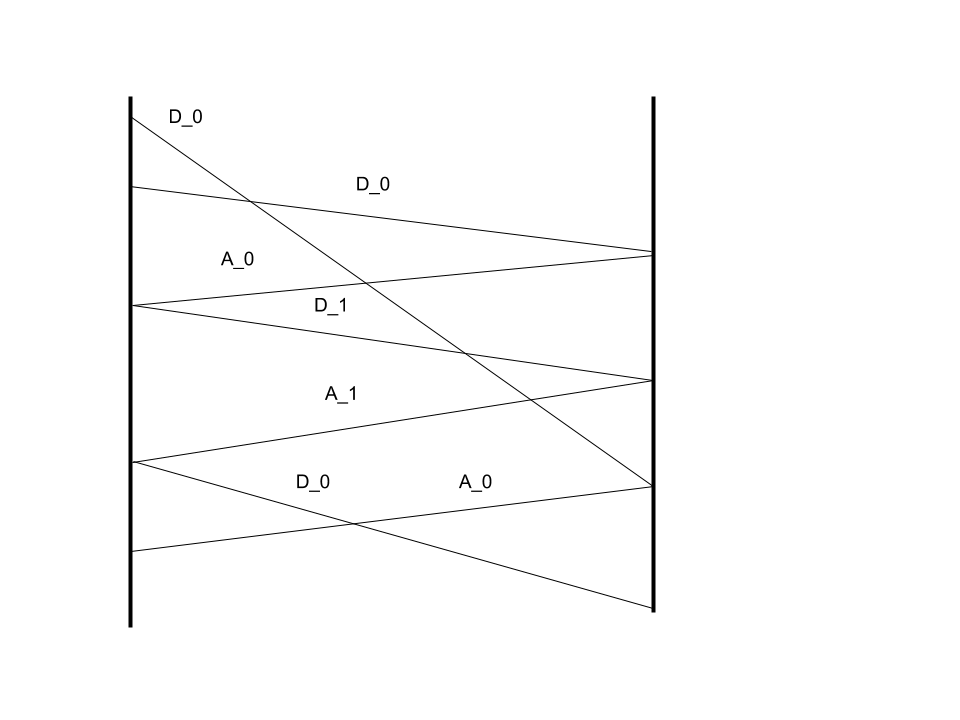
\includegraphics[scale=0.5]{P13}\\
If the initial D\_0 gets delayed so much and then arrives right after the receiver sends ACK1, the receiver will treat this as valid and send ACK0.  However, the receiver just send an ACK for a message that he has already received.  Thus this would not be reliable with only 2 sequence numbers


\item[P19.]
The FSM for the sender (A) would look as follows\\
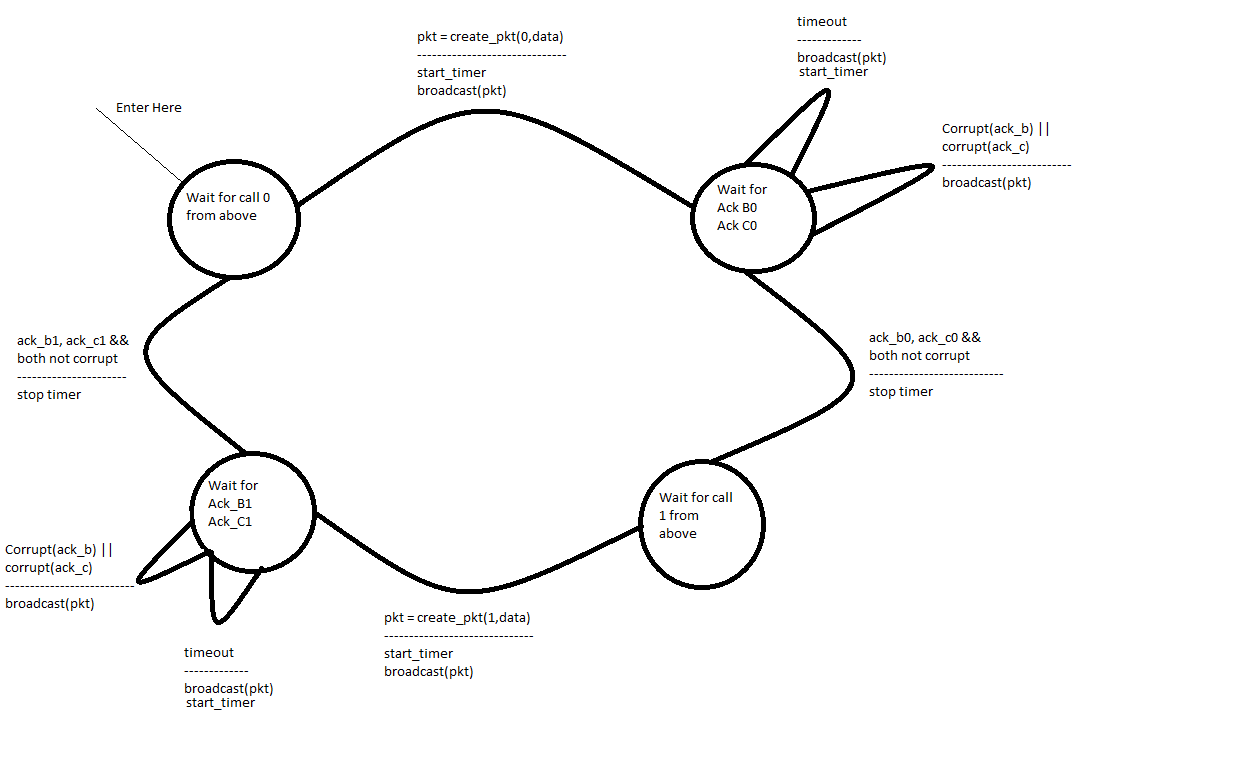
\includegraphics[scale=0.5]{p20_sender}\\
The sender will broadcast msg\_0 and start a timer.  If there is a timeout from either B or C, he will just rebroadcast the message.  If any of the Acks are corrupt, he will just rebroadcast the message.  If he recieves an ACK from either, he will store that information.  This way the ACK from the receiever only has to make it successfully once to A.  If both ACKs are not corrupt and received, he will proceeed to the next message\\
\newline
The FSM for the receiver (B or C) would look as follows\\
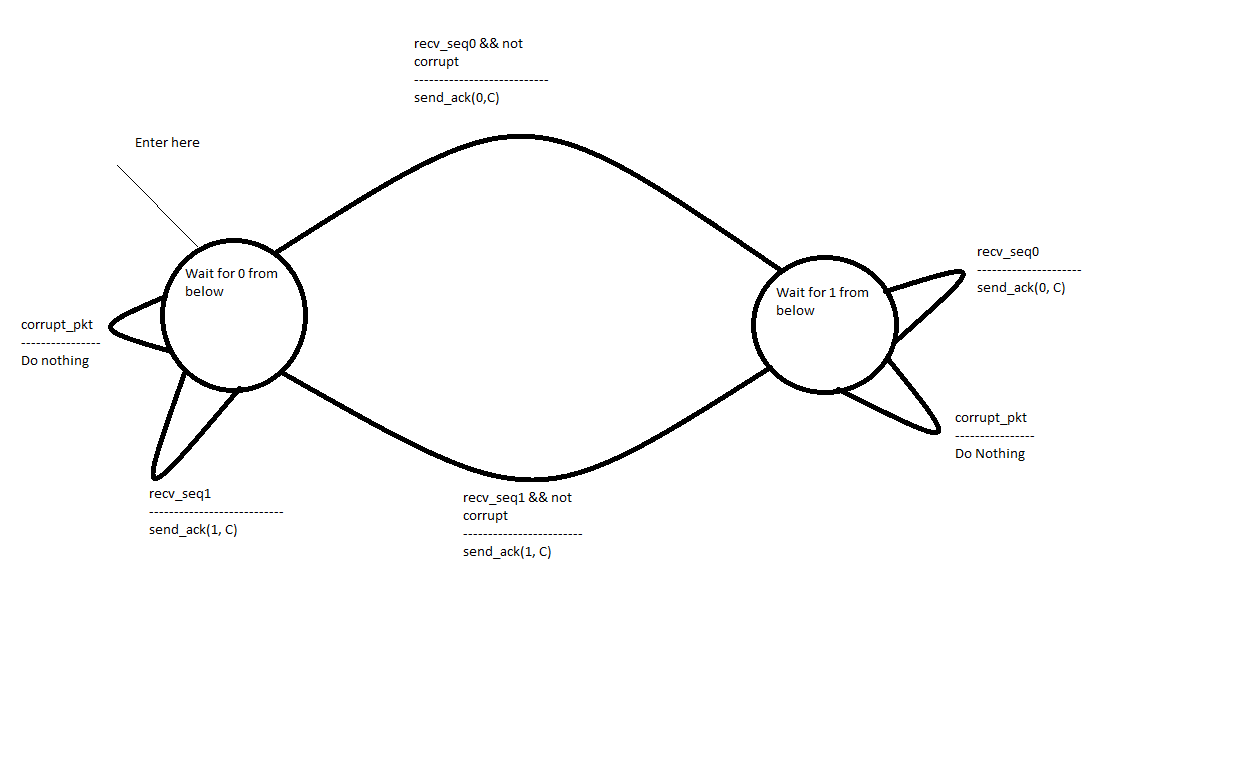
\includegraphics[scale=0.4]{p20_recv}\\
If receiver gets a corrupt packet, he just won't respond.  This will trigger a timeout and the packet will be rebroadcasted.  If he gets an out of order packet, he will just send an ACK for that packet.  This means that the previous ACK did not make it to the receiver.  When he recieves the correct packet that is not corrupt, he will send an ACK for that packet, along with his identity (B or C) and then wait for the packet next in the sequence\\
The packets will have to contain a sequence number, a checksum, a sender, and a receiver along with the data.

\item[P21.]
The FSM for the sender (A) would look as follows\\
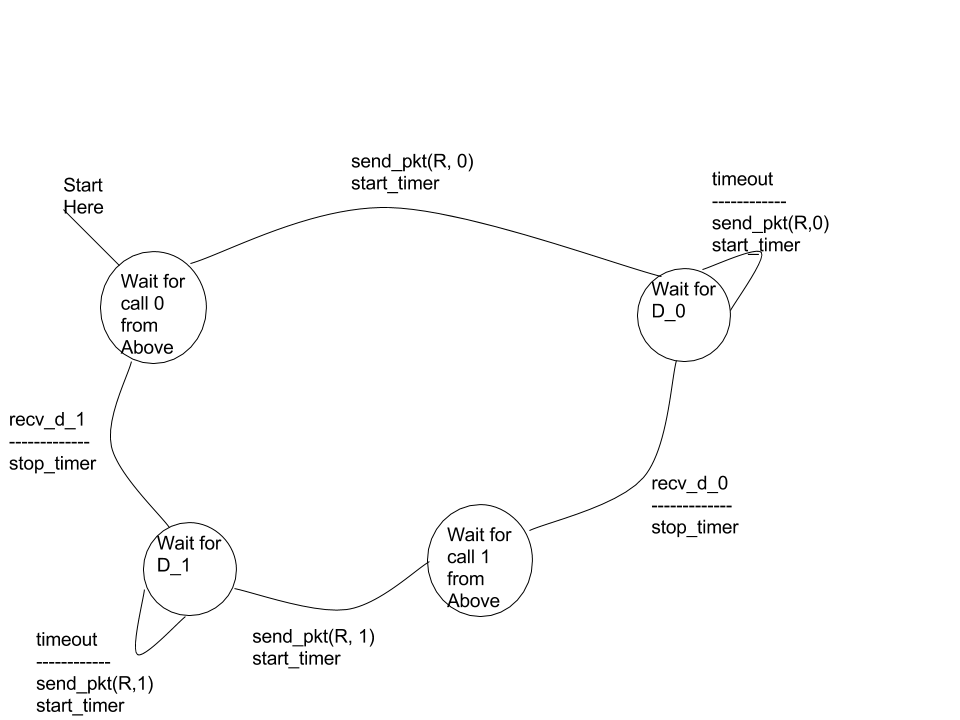
\includegraphics[scale=0.5]{p21_sender}\\
The sender will set an arbitrary timeout because the R packets can get lost.  As soon as he receives D0, then he can move on to R1.  He can send as many R packets as he wants because once the receiver gets even one of them, he will send the packets and ignore any R packets meant for the previous message\\
The FSM for the receiver (B) would look as follows\\
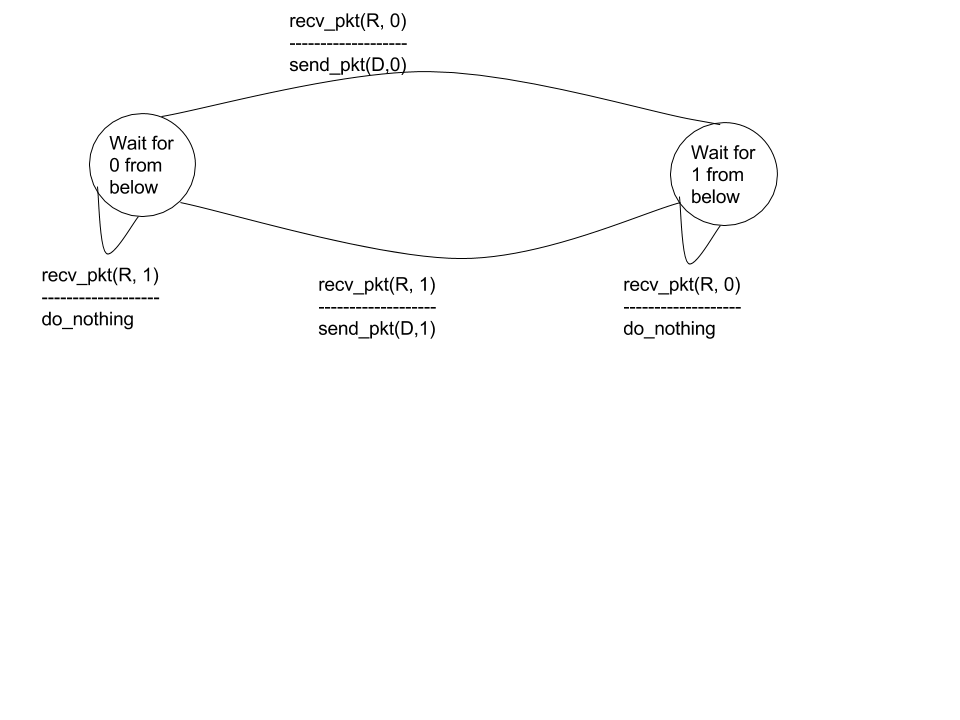
\includegraphics[scale=0.5]{p21_recv}\\
The receiver only cares are getting one R message for the current window state.  He knows that D will always make it to the sender, so once he send D, he can focus on only R messages of the next window.\\

\end{enumerate}

\section*{Answer 3}
\begin{enumerate}
\item[(a)] RTT = $270*2 = 540ms$, L/R = 1ms\\
Max utilization = $1 / 541 = .0018$

\item[(b)] Max seq number = 8.  This means we can only send 7 packets at a time\\
Max utilization = $.0018 * 7 = .013$
\end{enumerate}•

\end{document} 